\documentclass{article}
\usepackage[utf8]{inputenc}
\usepackage{amsmath}
\usepackage{amssymb}
\usepackage{graphicx}
\usepackage{minted}
\usepackage{biblatex}
\usepackage{hyperref}
\usepackage{siunitx}
\usepackage{pifont}
\newcommand{\cmark}{\ding{51}}%
\newcommand{\xmark}{\ding{55}}%
\addbibresource{ref.bib}

\title{Project Apicula}
\author{S.P. de Vos}
\date{October 2019}

\begin{document}

\maketitle

\tableofcontents

\section{Introduction}

During my Bachelor degree, I got in touch with FPGA development through several courses and projects. With my background in software development I was used to the best tools being open source and free to use, and was shocked that so much of the software used by electrical engineers is proprietary and inconvenient.

This project has the goal to add support for Gowin LittleBee FPGAs to an open source FPGA toolchain based around Yosys and Nextpnr. Adding support for more types of FPGAs is an important part of making Yosys and Nextpnr successful.

Here is a short summary of the contributions of this project to the open source FPGA landscape.

\begin{itemize}
    \item Improved synthesis support in Yosys for Gowin devices.
    \item Understanding of the hardware architecture used by Gowin FPGAs.
    \item Tools to parse database files provided by Gowin.
    \item Tools to extract complementary information from Gowin-generated bitstreams.
    \item An open source database that combines this data that can serve as the basis for many different open source programs.
    \item A proof-of-concept PnR flow based on this database.
    \item Tools for packing and unpacking bitstream files.
    \item A central repository of all the code, documentation, and database files at \url{https://github.com/pepijndevos/apicula/}
\end{itemize}

\subsection{FPGA internals}

\begin{figure}
    \centering
    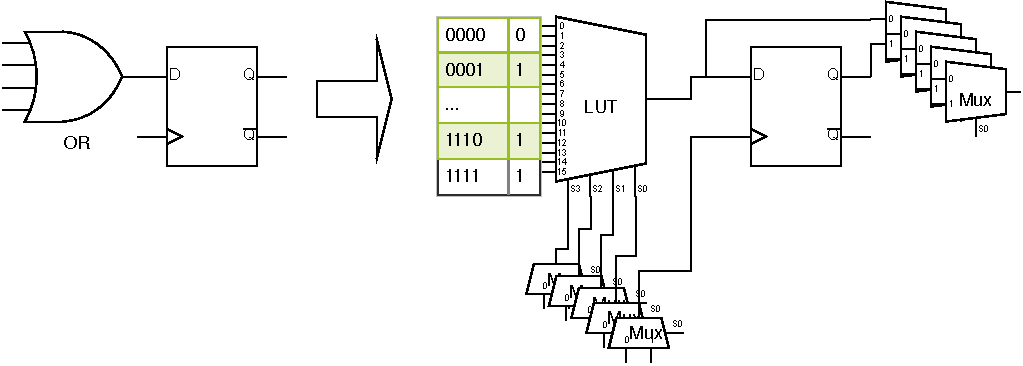
\includegraphics[width=\textwidth]{fig/slice.pdf}
    \caption{Schematic overview of an FPGA slice}
    \label{fig:slice}
\end{figure}

Before diving in what exactly has been done, it is important to understand how an FPGA works at a more abstract level. FPGA of course stands for field programmable gate array, so it appears there is an array of gates, and they can be programmed. But what does an array of gates look like, and how does one program one?

An FPGA is a digital logic device, so the fundamental building blocks are Boolean logic operations, clocked registers for making sequential programs, and wires to connect everything together.

Taking your classical Boolean operations such as AND, OR and XOR, you could make a truth table for each of them. Usually these operations have two inputs, but they can easily be extended to more inputs. More complex logic operations such as an adder can similarly be expressed as a truth table.

In FPGAs, these truth tables can be programmed into a lookup table, or LUT. This is basically a small piece of memory with only a small number of address lines and one bit of output. In most smaller FPGAs, LUTs with 4 address lines, and 16 bits of memory are used, but some larger FPGAs have LUTs with more inputs. The transformation of a 4-input OR gate to a LUT4 is demonstrated in figure \ref{fig:slice}.

A clocked register is implemented using a data flip-flop, or DFF. These propagate their input value to the output on a clock edge, and maintain the value until the next clock edge. They can usually also be initialised, reset, or disabled for more control.

To connect this all together, some sort of wiring between all these LUT and DFF is needed. Because it is infeasible to connect everything to everything, some structure is needed. The combination of a LUT and a DFF is grouped into a slice, and multiple slices are grouped into a tile. An FPGA is then a grid of tiles with wires between them.

In most FPGAs, there are wires within a tile, wires to the neighbouring tiles, and a few global wires for clock signals and the like. These wires are implemented using multiplexers, or MUX. A MUX selects between one of multiple inputs and drives one output. So each tile has a group of MUXes that select from the LUT and DFF outputs and incoming wires from neighbouring tiles, and drive local LUT/DFF inputs and wires to neighbouring tiles. The structure of a Gowin tile is shown in figure \ref{fig:wiring}.

In addition to those basic building blocks, FPGAs contain many other special-purpose tiles. There are I/O buffers (IOB) around the edges to interface with the outer world, there are phase-locked loops (PLL) for generating clock signals, there are hardware carry chains for fast arithmetic, there are DSP tiles for multiply-accumulate operations common in digital signal processing, there are block RAM (BRAM) tiles for storing data, and many more.

So to configure an FPGA then, it is needed to configure all these LUT bits, MUX inputs, and other tiles. This is done by loading a bitstream from a piece of flash memory and into the FPGA. These bitstreams are generated by the vendor toolchains, and their format is not documented. The goal of this project is to document the format of one such bitstream.

\subsection{Software landscape}

To generate these bitstreams, a lot of software is needed. First a program written in a hardware description language (HDL) such as Verilog, VHDL, Clash\cite{clash}, Chisel\cite{chisel}, nMigen\cite{nmigen}, etc. needs to be synthesized to a netlist of these basic building blocks described above. This netlist then needs to be mapped to the available LUTs, DFFs, MUXes, and other resources available on the FPGA. And finally the annotated netlist needs to be converted to an actual bitstream.

Traditionally, all these functions are performed by proprietary software, produced by the vendor of a specific FPGA, but open source alternatives are on the rise, providing an unified feature set across all FPGA devices, and allowing endless customization and integration.

Figure \ref{fig:symbiflow} shows an overview of the open source toolchain. The frontend is what reads HDL, and based on architecture definitions of the vendor's primitives, generates a low-level netlist. The backend can be either post-synthesis simulation of the netlist, or generating a bitstream using either Nextpnr or VTR\cite{Rose:2012:VPA:2145694.2145708}, with the corresponding architecture definition of the desired FPGA type.

Figure \ref{fig:symbiflow2} shows how the various tools interoperate with each other using various intermediate representations. On the left are various HDL file formats, which can by synthesized using Yosys, Quartus, or any other synthesis tool, producing a netlist format such as blif, json, edif, etc. These can then be fed to open source PnR tools such as Nextpnr, or proprietary ones such as Vivado. The open source tools then produce a low-level description of all the primitives and locations used, which can again be programmed to the FPGA using either open source or proprietary tools.

\begin{figure}
    \centering
    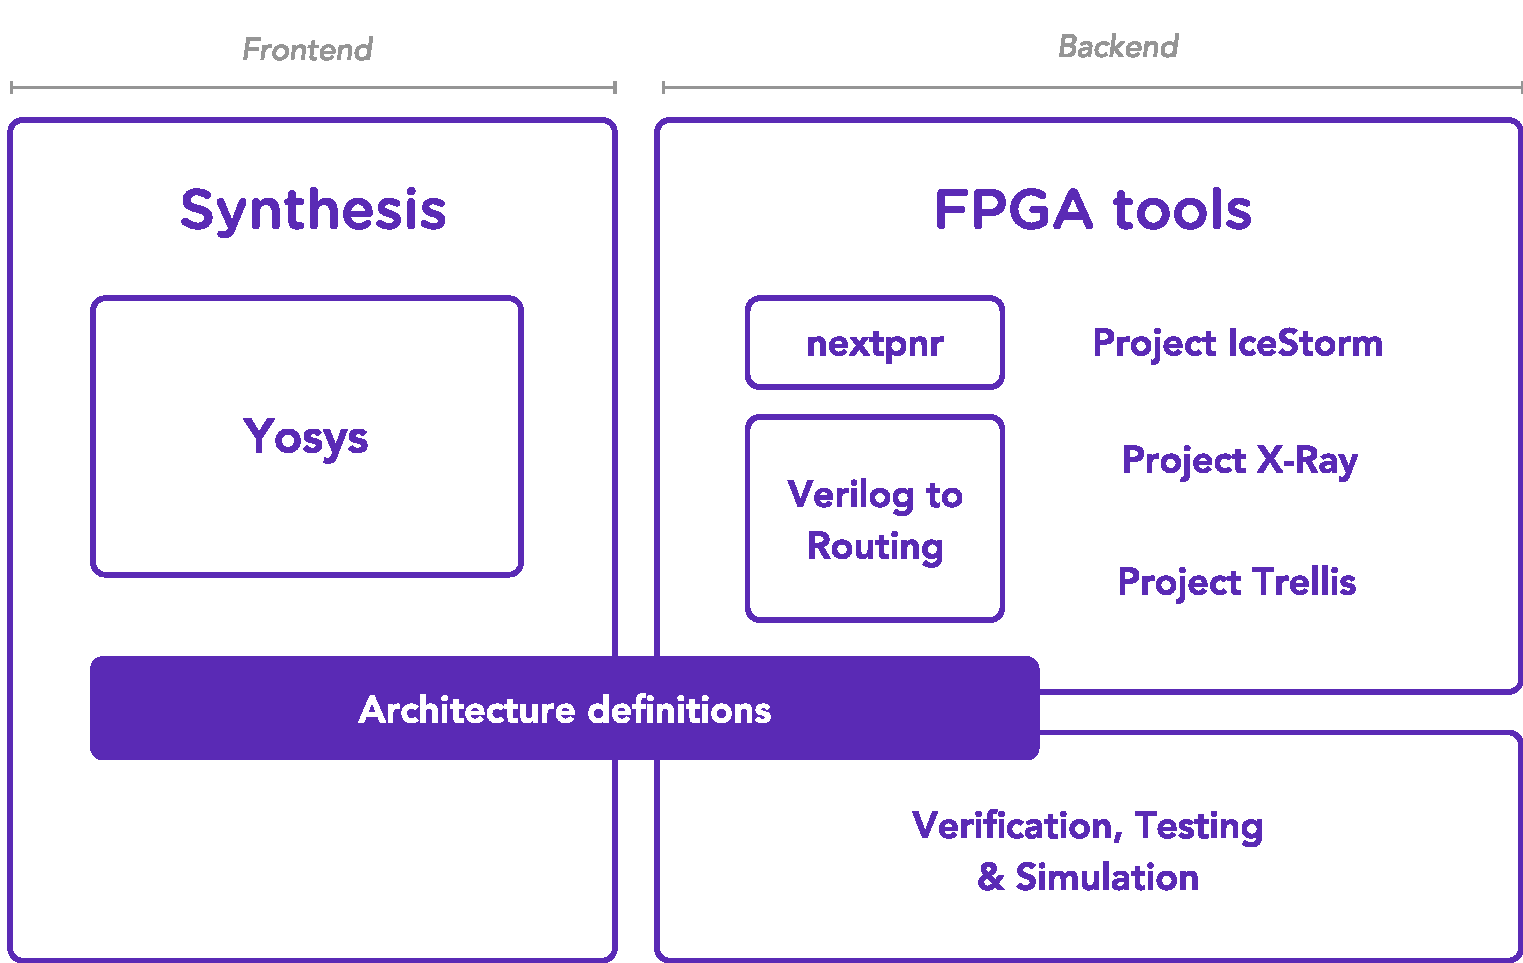
\includegraphics[width=\textwidth]{fig/parts.pdf}
    \caption{An overview of the open source toolchain \cite{symbiflow}}
    \label{fig:symbiflow}
\end{figure}

\begin{figure}
    \centering
    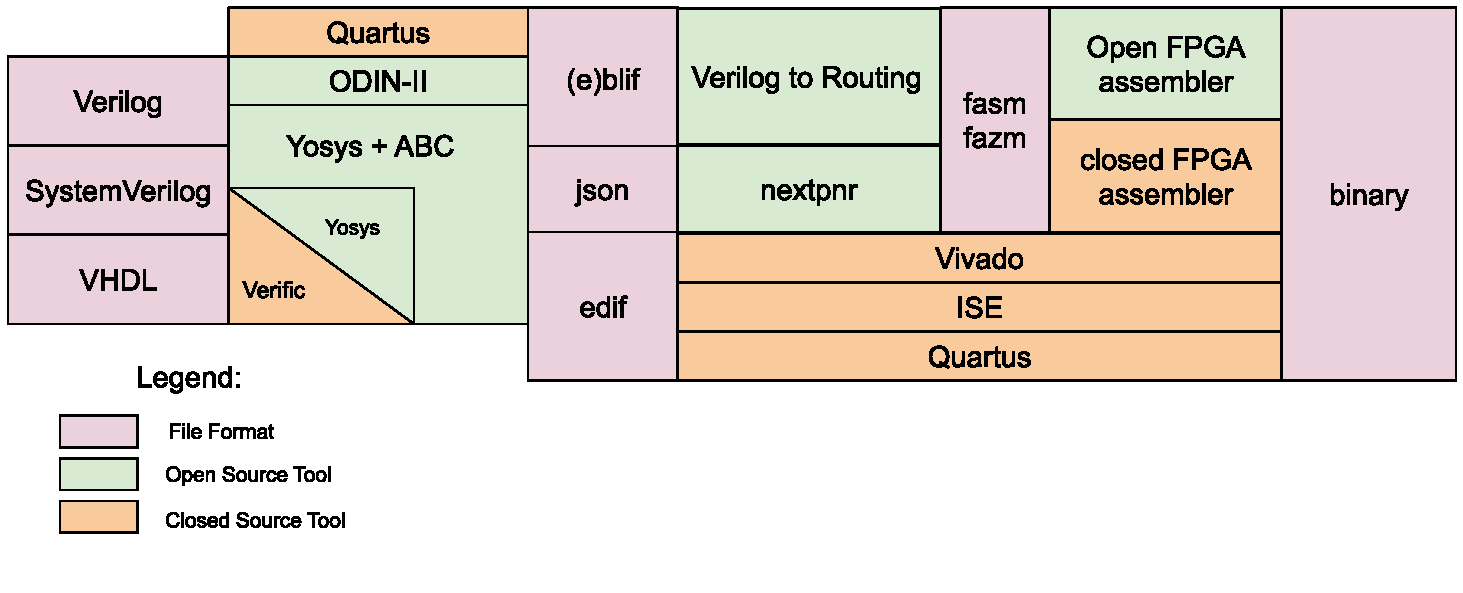
\includegraphics[width=\textwidth]{fig/toolchain-flow.pdf}
    \caption{Possible routes from HDL to bitstream \cite{symbiflow}}
    \label{fig:symbiflow2}
\end{figure}

Yosys is an open source synthesis tool originally developed by Clifford Wolf for the Icestorm project. It is a very flexible compiler based on a command architecture. This allow you to compose different commands to do specific things, and add new commands for specific input and output formats.

For end users the primary commands are \texttt{read\_*} (\texttt{read\_verilog}, etc.) and the \texttt{synth\_*} (\texttt{synth\_ice40}, etc.) commands, which pares HDL code into RTLIL (register transfer level intermediate language), and then uses the FPGA architecture description and various sub-commands to generate an FPGA-specific netlist. Sub-commands include compiling sequential processes to flip-flops, mapping Boolean logic to lookup tables, mapping generic cell types to FPGA-specific ones, and various optimization passes.

Yosys can output various netlist formats for usage with simulators, formal verification, vendor PnR tools, and the open source PnR tools. In the case of Nextpnr, used in this report, a JSON format is used.

Synthesis produces a netlist of interconnected vendor primitives. However, an FPGA has these primitives laid out in a grid with connections to adjacent tiles. So it is of crucial importance for the area, power, and speed of a design, to place the primitives in such a way that they can be easily connected, and to use the shortest possible connection. This is in a nutshell what place and route is all about.

For place and route, there are two main open source tools. The oldest one is VTR\cite{Rose:2012:VPA:2145694.2145708} (verilog to routing), a research tool to design and test new theoretical FPGA architectures. It uses an XML based format to describe an FPGA. Some people believe that VTR is not well suited to describe the warts and kinks of real-world commercial FPGAs, so they wrote another PnR tool called Nextpnr, which uses programmatic descriptions on FPGA architectures, and is written from the ground up with commercial FPGAs in mind.

Both PnR tools rely on separate bitstream documentation projects that document the architecture of a class of FPGAs, and produces a so called ChipDB that is a machine-readable description of an FPGA. Project Apicula is such a project, which aims to provide a ChipDB for Gowin FPGAs. Other projects include IceStorm\cite{IceStorm} for Lattice iCE40 FPGAs, Project Trellis\cite{Trellis} for Lattice ECP5 FPGAs, and Project X-Ray\cite{xray} for Xilinx 7 Series FPGAs.

When discussing Nextpnr, it is prudent to establish some terminology \cite{nexpnrfaq}. A netlist consists of cells connected by nets. An FPGA consists of bels (basic elements), connected by wires and pips (programmable interconnect points). The goal is to map cells and nets to bels and pips, this is done in 3 stages.

First, packing combines HDL ``primitives'' into larger items such as a slice that contains both a LUT and DFF. After packing, there is a one-to-one correspondence between cell types and bel types. Then, placement places these cells on available bels in the FPGA. Finally, routing uses pips to connect the bels together.

Originally, placement was done using successive approximation, an iterative approach that works relatively well for small FPGAs. But at the moment, placement can also be done using an analytical placer that scales much better to medium and large FPGAs.

\subsection{Problem analysis}

Programming an FPGA consists of several steps. First a HDL (hardware description language) design is synthesized to a netlist by a tools such as Synopsys Synplify or Yosys. This step only requires information about the FPGA architecture and available primitives. So adding a new FPGA to Yosys is fairly straightforward in most cases.

After that a place and route step is done that maps the generated netlist to the available hardware on the FPGA. This requires understanding of the hardware blocks and interconnections between them. This information is only partially published through documentation and the floorplanner, but much of the needed information needs to be derived by other means.

The final step is that a binary bitstream file needs to be generated to program the routed design onto the FPGA. This binary format is completely undocumented, and also needs to be derived through other means.

When I started, partial support for Gowin FPGAs was already implemented in Yosys. This means a HDL design can be synthesized using Yosys, but the resulting netlist has to be run through the vendor place and route tools. It also lacks support for some advanced resources such as ALU carry chains and DSP blocks, meaning they are slower and take up more space than needed.

The tools for place and route and bitstream generation are completely missing and have to be developed by inspecting the official vendor tools.

In summary, what needs to be done is first of all, discover the internal architecture and bitstream format of the FPGA. This will be the majority of the work. Based on this, Yosys support can be improved, a Nextpnr target can be added, and a bitstream packer can be written. However, Yosys support already exist and does not require a deep understanding of the FPGA internals, so it is a good place to start.

\section{Synthesis}

As mentioned, Yosys is a synthesis tools that reads HDL and produces a netlist based on a series of commands that read, modify, optimize, and write the program. To support synthesis for Gowin FPGAs, a \texttt{synth\_gowin} command needs to be added that can produce Verilog compatible with the vendor tools. This requires writing descriptions of the vendor primitives and commands to translate HDL to the vendor format.

When the project started, there was already preliminary support for Gowin in Yosys. However, it was found that the existing support was not up to date with the most recent version of the vendor tools. Through reading documentation and experimenting, the Gowin support in Yosys was fixed to work with Gowin IDE 1.9, and was further extended.

\subsection{Primitives}

\begin{table}[]
\caption{Yosys- and vendor primitives}
\label{tab:vendor-prims}
\begin{tabular}{|l|l|l|}
\hline
\textbf{Yosys primitive} & \textbf{Vendor primitive}   & \textbf{Function}                                     \\ \hline
\$dff, \$adff              & DFF{[}N{]}{[}SRPC{]}{[}E{]} & A data flip-flop \\ \hline
\$and, \$or, ...           & LUT{[}1-4{]}                & A lookup table for binary logic           \\ \hline
\$alu                    & ALU                         & Arithmetic with hardware carry chain                  \\ \hline
\$macc                   & PADD, MULT, ...             & DSP multiply-accumulate primitives                    \\ \hline
N/A                      & IBUF, OBUF, ...           & A a physical I/O pin     \\ \hline
\$memrd, \$memwr           & SP, SDP, DP, ...            & Block-RAM primitives                                  \\ \hline
\end{tabular}
\end{table}

An important part of synthesis is technology mapping, which takes generic primitives whose names start with a dollar sign \cite{yosysman}, and translates them to vendor-specific primitives. This is done by writing a specially crafted Verilog file with parameters that indicate the replacement that is done. This file is applied with the \texttt{techmap} command.

The vendor provides a document with all their primitives \cite{gowinprim}, of which some parts are summarised in table \ref{tab:vendor-prims}, what follows is a description of some items, the improvements that were made and implementation challenges faced.

The existing flow provided a simple mapping from \texttt{\$dff} to a few vendor variatons of \texttt{DFF}. However, the vendor provides dozens of different types with \texttt{E} (clock enable), \texttt{N} (negative clock), \texttt{S} (synchronous set), \texttt{R} (synchronous reset), \texttt{P} (asynchronous preset), \texttt{C} (asynchronous clear), and combinations of those.

For all these combinations, simulation models, tests, and techmaps were written, and commands written to map to them. A challenge was that the vendor supports an \texttt{INIT} parameter that sets the initial value of the DFF. Partial support for this existed, but it was found that the hardware does not actually support initial values. Instead, the DFF is initialised to its reset value, so what the vendor tool does when an initial value is used, is to synthesize a DFF with the correct reset type with the reset tied low. This was mimicked in the techmap file using \texttt{generate} blocks.

The existing flow already provided \texttt{LUT1} to \texttt{LUT4} types, however, Gowin has the capability to combine LUTs together with a MUX. This way, two \texttt{LUT4} and a \texttt{MUX2\_LUT5} can be combined to form a LUT with 5 inputs, and two of these can again be combined with a \texttt{MUX2\_LUT6} to form a LUT with 6 inputs. This can be done up to 8 inputs.

A challenge with adding wide LUTs is that ABC, a tool that maps Boolean logic to LUTs, does not have a detailed understanding of the timing delays of the MUXes, making it overly eager to use wide LUTs. A new experimental version of ABC can use detailed timing models to make a better estimate, but such models are not available for Gowin yet.

The \texttt{MUX2} primitive can also be used on its own as a multiplexer, which was implemented initially but then removed again because it produced worse result. By mapping MUXes to vendor primitives, ABC can no longer optimize them when converting logic to LUTs. This reduced room for optimization makes for worse results. It also appears that the configurations in which a \texttt{MUX2} can be used are fairly limited, causing the FPGA to run out of space for even fairly modest designs.

Yosys has an \texttt{\$alu} cell that implements addition and subtraction, and indirectly, comparisons. It has a \texttt{BI} input that inverts the \texttt{B} input for subtraction. The existing pass used the vendor primitive in the \texttt{ADD} mode, adding an external inverter for subtract. This was updated to use the \texttt{ADDSUB} mode which has a similar "invert B" input, saving an extra inverter per bit on the FPGA. The vendor ALU supports more types, but there is no clear way to use them in a beneficial way with Yosys.

Gowin supports both distributed RAM and block RAM. Distributed ram uses a LUT as an actual memory with some extra wires, existing support exists for one types, and this was not changed. Block ram supported a few configurations, which was expanded upon. BRAM blocks can be used in various data widths and address widths, of which the largest was not yet implemented. The two widest modes support a byte-enable allowing to write parts of a word only, so that was added as well. The key thing that was added is memory initialisation, which required writing a Python script to generate the correct list of parameters.

An implementation challenge with BRAM is that while the vendor supports single port RAM, semi dual port RAM, and true dual port RAM, Yosys currently only supports semi dual port RAM. Single port RAM is not supported because Yosys requires a separate read and write port, so it cannot work with only one port. The difference between semi- and true dual port RAM is that true dual port RAM has two seperate clock domains for the read and write port. Sadly, Yosys does not yet support inferring BRAM across different clock domains.

Gowin also supports latches and DPS blocks, but these are not yet supported. Other primitives such as LVDS and PLL cannot be inferred by Yosys at all and require manual instantiation.

\subsection{Passes}

\begin{figure}
    \centering
    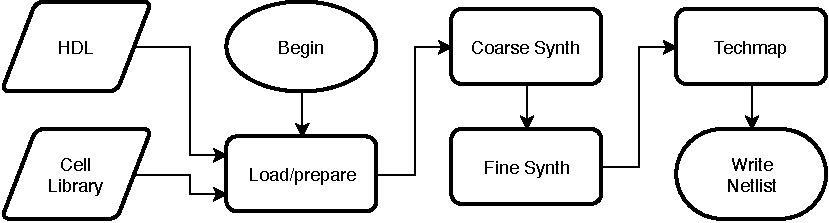
\includegraphics[width=\textwidth]{fig/synthflow.pdf}
    \caption{Yosys Synthesis flow}
    \label{fig:synthflow}
\end{figure}

As explained, Yosys uses a sequence of smaller compilation passes that can be composed in various ways. Below is an overview of the key steps in the \texttt{synth\_gowin} command, of which the sub-steps are shown in figure \ref{fig:synthflow}: the design is loaded, translated to coarse word-level cells, which are mapped to fine bit-level cells, which are mapped to vendor primitives, and written out to a netlist.

First it uses \texttt{read\_verilog -lib} to load the simulation models as "blackbox" (no implementation) primitives. Then it does coarse synthesis, which uses some commands to flatten the design, convert processes to logic, followed by \texttt{synth -run coarse} which runs part of the generic synthesis script to do some optimizations on the design. Then it executes \texttt{memory\_bram} to infer BRAM and DRAM using a textual description of the vendor primitives.

Next it does fine synthesis, which contains further optimizations and map specific cells such as \texttt{\$alu} to vendor primitives imported earlier. One addition that was made here was to add a \texttt{splitnets} to split nets into individual bits, due to vendor limitations. First there are some passes that map coarse \texttt{\$dff} cells to fine \texttt{\$\_DFF\_} cells with specific characteristics such as their clock polarity, clock enable, and reset behaviour encoded in their name. Then it converts all Boolean logic to LUTs. This is done by an external program called ABC. What was added here is the option to use or disable wide LUTs (which ABC is overly eager to use), and the option to use the experimental ABC9 (without proper timing models unfortunately).

The penultimate step is to map the bit-level fine cells to vendor primitives, which is done in the final \texttt{techmap} phase. This phase also maps top-level ports to vendor I/O buffer cells, and drives undefined wires low to avoid errors from the vendor tool.

And then finally some final checks are executed to make sure things are not obviously broken, and some statistics are printed about how many cells are used.

\section{Documenting}

With working Yosys support, HDL designs can be synthesized using Yosys, and then placed and routed using the vendor tool. While this allows easier code sharing between FPGA architectures, proprietary software is still needed to do PnR and program the FPGA. For a full end-to-end open source flow, the internal FPGA architecture and bitstream format need to be documented.

For extracting the information needed to do PnR and generate a bitstream, there are several methods. First and foremost is just collecting all the information the vendor tools give you. For many vendors this includes information about routing, but in the case of Gowin, hardly any useful information is generated in the PnR phase besides the actual bitstream.

\subsection{Fuzzing}

The preferred method of extracting data about the bitstream is fuzzing. This means that and automated system runs the vendor PnR tools on many different generated netlists and correlates the configuration of primitives in the netlist to bits in the bitstream.

The basic idea is that you take a program, generate a bitstream, change one tiny element of the program and generate another bitstream. The difference between the two bitstreams then tells you which bits are related to that particular feature.

I started by writing bash scripts to generate simple netlists with sed and then running the vendor TCL shell to generate a bitstream. Different netlists were then compared in a Python script that would generate an image. However, after talking to a fuzzing expert at the company, I was recommended to take a more integrated and sophisticated approach.

There are two different approaches to fuzzing. One where you first determine the tile grid layout, and fuzz a single tile. The other just fuzzes every bit in the whole FPGA as efficiently as possible. The latter is more complex, but requires less prior knowledge and has the added benefit that it detects unexpected interdependencies that might not show up if you turn one feature on or off at the time.

The second iteration of the fuzzer is of the whole-FPGA kind, and completely written in Python. A fuzzer is defined as a python class that uses a code generation module to generate netlists on the fly. These are then saved in temporary directories where the vendor tools are run in parallel to utilize all CPU cores. The results are then read and a report of all bitstream locations is generated.

Rather than fuzzing one bit at a time, the new fuzzer uses a system where $N$ bits can be found in $\log_2(N)$ PnR runs, by changing each bit in an unique pattern. For example, a run with 8 configuration bits could be done in 3 runs using patterns $00001111$, $00110011$, $01010101$ as shown in table \ref{tab:binarycodes}. However, in reality a fuzzer can test thousands of bits at a time, requiring about 20 PnR runs per batch to locate all of them. Multiple batches are needed to test incompatible fuzzers that use the same resources.

\begin{table}[]
\centering
\caption{Binary codes}
\label{tab:binarycodes}
\begin{tabular}{r|ccccccccc}
\textbf{Run\textbackslash bit} & \textbf{A} & \textbf{B} & \textbf{C} & \textbf{D} & \textbf{E} & \textbf{F} & \textbf{G} & \textbf{H} & \textbf{B$\parallel$C} \\ \hline
\textbf{1}       & 0          & 0          & 0          & 0          & 1          & 1          & 1          & 1          & 0            \\
\textbf{2}       & 0          & 0          & 1          & 1          & 0          & 0          & 1          & 1          & 1            \\
\textbf{3}       & 0          & 1          & 0          & 1          & 0          & 1          & 0          & 1          & 1            \\ \hline
\textbf{Unique}  &\textbf{\xmark}&\textbf{\cmark}&\textbf{\cmark}&\textbf{\cmark}&\textbf{\cmark}&\textbf{\cmark}&\textbf{\cmark}&\textbf{\xmark}&\textbf{\xmark}             
\end{tabular}
\end{table}

In the above example, the first feature would generate a bit pattern of $000$ across the three runs, while the second would have the bit pattern $001$, and the last one will have $111$. The first and last ones are problematic because all bits that are not involved in the test are also all zero or all one. Another problem shows up with bits that are not 1:1 relations to program features. (one example is I/O buffer bank enable that are set if \textit{any} pin in that bank is used) These features generate different codes that may correspond to another unrelated feature.

To avoid all-zero and all-one codes and to detect codes that do not correspond 1:1 to a tested feature, the fuzzer uses constant Hamming weight codes rather than straight binary. Hamming codes have a constant number of ones and zeros, which means that in most cases it can detect codes due to unexpected side effects. The same 8-bit example is displayed with Hamming codes in table \ref{tab:hammingcodes}. Note that it takes more runs, but the OR of bits B and C produce an unique code.

To correctly handle side-effects such as bank-enable bits on toggling an output pin, meta-fuzzers were introduced. A meta-fuzzer exposes a list of extra codes it expects given the configuration bits given to the fuzzer. It also produces groups of bits that toggle a particular extra bit, which are use to generate additional PnR runs to detect them. For example, D$\parallel$E would be 11111 and not be detected properly, so an additional run with both D and E zero needs to be generated.


\begin{table}[]
\centering
\caption{Hamming codes}
\label{tab:hammingcodes}
\begin{tabular}{r|ccccccccc}
\textbf{Run\textbackslash bit} & \textbf{A} & \textbf{B} & \textbf{C} & \textbf{D} & \textbf{E} & \textbf{F} & \textbf{G} & \textbf{H} & \textbf{B$\parallel$C} \\ \hline
\textbf{1}       & 0          & 0          & 0          & 0          & 1          & 1          & 1          & 1          & 0            \\
\textbf{2}       & 0          & 1          & 1          & 1          & 0          & 0          & 0          & 0          & 1            \\
\textbf{3}       & 1          & 0          & 1          & 1          & 0          & 1          & 1          & 1          & 1            \\
\textbf{4}       & 1          & 1          & 0          & 1          & 1          & 0          & 1          & 1          & 1            \\
\textbf{5}       & 1          & 1          & 1          & 0          & 1          & 1          & 0          & 0          & 1            \\
\textbf{Unique}  &\textbf{\cmark}&\textbf{\cmark}&\textbf{\cmark}&\textbf{\cmark}&\textbf{\cmark}&\textbf{\cmark}&\textbf{\cmark}&\textbf{\cmark}&\textbf{\cmark}             
\end{tabular}
\end{table}

This fuzzer is sufficient to find bits for most cell types, such as lookup tables, flip-flops, and I/O buffers. However, a major challenge was hit in routing. Unlike most other vendors, the Gowin tools do not give any indication or control over which wires are in use, or even which wires exist at all. According to experts at the company, this makes fuzzing Gowin routing several orders of magnitude harder than previous efforts, despite the FPGA otherwise being relatively simple. Because of this, ChipDB decoding was used in addition to fuzzing as explained in \ref{sec:chipdb}.

After the ChipDB was decoded, a third fuzzer was written of the one-tile-at-a-time kind. Since the tile types and boundaries were now known, a very simple fuzzer could be written that fuzzes a single item per tile. Where the second fuzzer required complex code and long run-times, the third fuzzer is less than 200 lines of code and runs in under a minute. It also directly records results in a machine-readable database, together with information from the vendor files.

\subsection{ChipDB decoding}\label{sec:chipdb}

Another approach to obtain information about the PnR resources and bitstream format is through decoding the data files known as the chipDB that ship with the vendor tools. These files directly contain the resources, layout, and bitstream format of all FPGAs supported by then vendor. 

To decode the chipDB, first GDB was used to set a catchpoint on the \texttt{openat} syscall to determine the functions where the files are read. This function was then decompiled with Ghidra to see how it is read. From there GDB is used again. In one case data was read into a struct, and GDB watchpoints were used to connect getter methods to struct offsets. In another case a class-based archive format was used, where a GDB breakpoint on \texttt{fread} was used to connect class names to file offsets.

Once the format had been figured out, a Python parser was written to extract the data for further use. One of the first uses was to generate images in the same format as the fuzzer, so fuzzing results can be compared to chipDB results. Then other tools were written, directly using the vendor ChipDB.

Even with the decompiled parsing code, attaching meaning to the data was a big challenge. A major roadblock was that the routing information used wire IDs with unknown meanings. While some guesses could be made about their general usage, no exact routing table could be derived from the data file. Another foray into decompiled code was needed to locate the names of these wires. They were generated with some extremely hard to follow C++ code that wrote them to a vector. Eventually some long GDB command was used to extract the generated vector from the running program.

With these wire names in hand, some guesses could be made and then verified about the meaning of the data in those files. A table of wires was found, which for each wire contained the fuses to set. These fuses are indexes into a table, that combined with the tile type, give a 4-digit decimal number of the format \texttt{YYXX} which encodes the location of a bit to set relative to the top-left of the tile.

The same format was used for data tables that appear to contain info about LUTs, DFFs and IOBs. Since these results were previously known from fuzzing, they could be cross-checked for correctness. However, a very puzzling thing was that there were negative wire numbers and features in these tables. It was found that for wires, these indicate the default state of a MUX, so if the specified fuse \textit{is not} set, then these wires are connected.

\subsection{FPGA Architecture}

Gowin FPGAs have a LUT4 architecture common to many smaller FPGA architectures. The FPGA consist of a grid of tiles with I/O buffers around the edges, rows of special-function blocks such as BRAM, and a large grid configurable logic units.

Figure \ref{fig:tiles} gives an overview of the tiles on a small Gowin FPGA. All the tiles labeled CFU are normal logic tiles. The row below BRAM are also logic tiles, but with different connections. All edges except the PLL and corner tiles are I/O buffers, but the IOB in the centers are a bit different. One BRAM is 3 tiles wide, hence the alternating pattern. The central tiles are in fact not BRAM and are used in global clock routing and other functions.

\begin{figure}
    \centering
    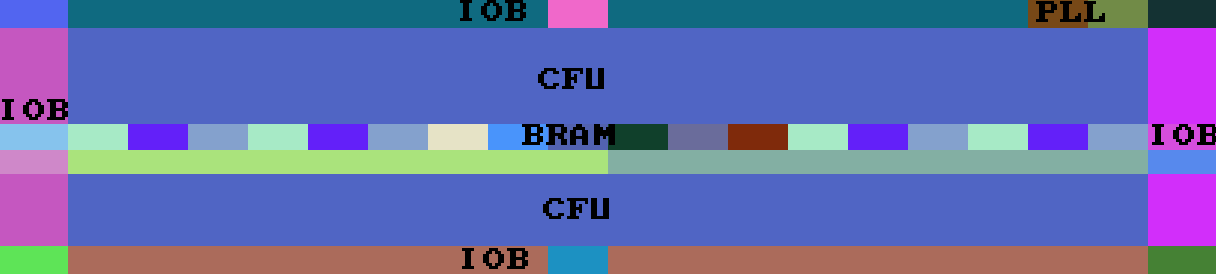
\includegraphics[width=\textwidth]{fig/fuse.png}
    \caption{Tile layout for GW1N-1}
    \label{fig:tiles}
\end{figure}

Each Configurable logic unit consists of 8 LUT4s grouped in 4 slices, of which 3 have data flip-flops. Each slice shares certain resources such as clock inputs and reset lines.

Each LUT4 has 4 inputs and one output that is directly connected to the data flip-flop input. The LUT output can be used independently, but the flip-flop is always used through the LUT. Each pair of flip flops has data in and out, clock, clock enable, and set/reset. Each pair of flip-flops can be configured for rising edge or falling edge sensitivity, and asynchronous or synchronous set or clear.

These tiles are connected with various multiplexers to adjacent tiles as well as global clock lines. Each tile has 8 tile-local wires, and in each direction it has 4 one-hop wires of which 2 are shared between north/south and east/west, 8 two-hop wires with one-hop taps, and 4 eight-hop wires with four-hop taps. An overview of all wires can be seen in Figure \ref{fig:wiring}.

\begin{figure}
    \centering
    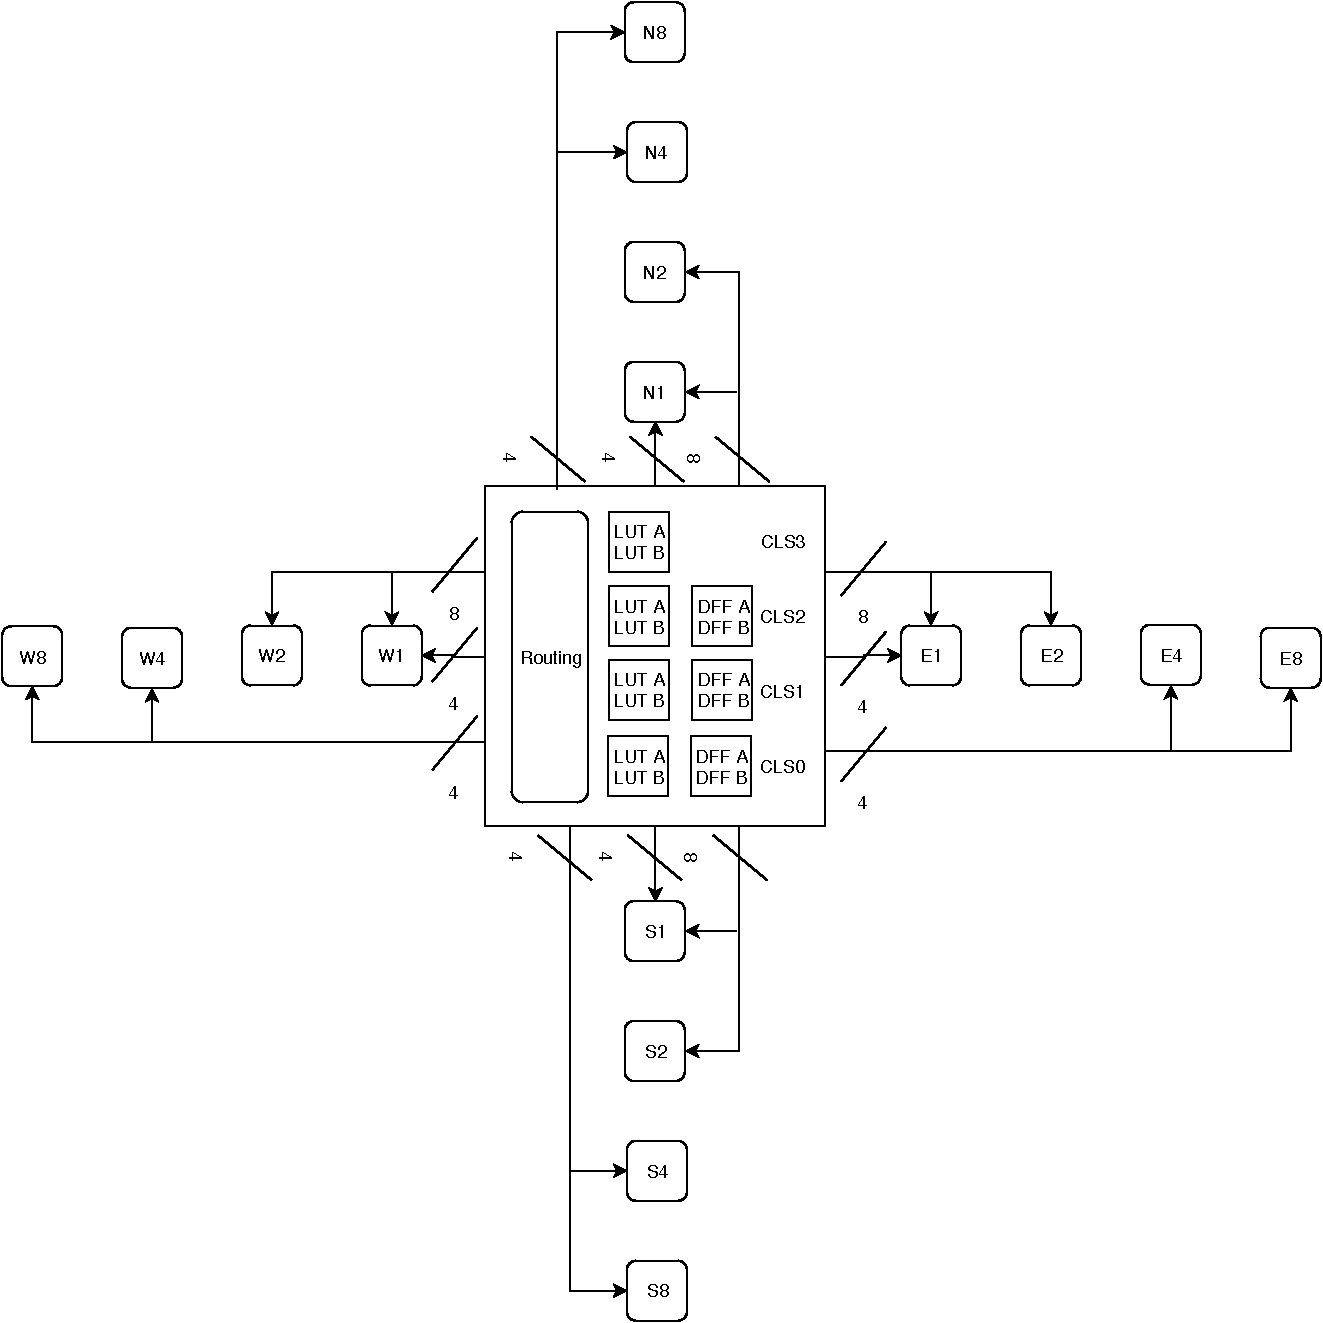
\includegraphics[width=\textwidth]{fig/clu.pdf}
    \caption{Tile structure and wires}
    \label{fig:wiring}
\end{figure}

\subsection{Bitstream Structure}

Gowin outputs a bitstream in ASCII binary notation, making it easy to separate commands form data frames.

Data frames describe one row of bits on the FPGA tile grid. Frames are padded to full bytes, and verified with a CRC-16 checksum. These rows are stacked on top of each other to describe a bitmap that is overlaid on the FPGA tile grid.

The number of tiles on the grid depend on the specific FPGA model. A tile is roughly $60\times24$ bits, with I/O buffers and some special tiles being a few rows or columns larger. A common logic tile has the LUTs and flip-flops in the bottom 4 rows, with the top 20 rows being filled with multiplexers. An overview of the bitstream layout of LUTs, flip-flops, and multiplexers in a logic tile can be seen in Figure \ref{fig:bits}.

\begin{figure}
    \centering
    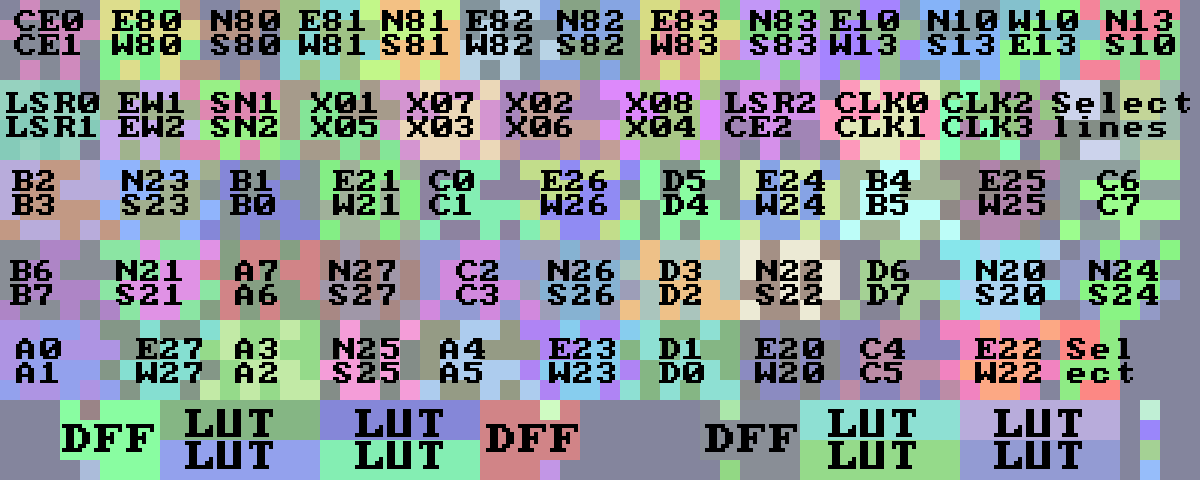
\includegraphics[width=\textwidth]{fig/tile.png}
    \caption{Logic tile bits. Each colour corresponds to a single MUX or other primitive. MUX labels indicate the destination wire of the MUX.}
    \label{fig:bits}
\end{figure}


\section{Place and Route}

Once the structure of the FPGA is understood, software can be written to parse and generate bitstreams. It was decided to start with the unpacker and initially focus on a bare minimum flow with just basic logic, wires, and I/O ports.

FPGA's contain many special purpose hardware blocks that are desirable to support eventually, but it is better to have something working and then make it perfect later. The main things that are needed are lookup tables for logic, flip-flops for sequential steps, wires to connect things together, and I/O buffers to connect to external FPGA pins.

The first part of the PnR tools that was written is the unpacker, which transforms a bitstream back to code. This allows to validate our understanding of the bitstream by comparing post-synthesis netlists with unpacked netlists from bitstreams generated by the vendor PnR tools. It is also an important debugging tool for debugging the output of the open source PnR tools.

Before full-fledged support for all aspects of the FPGA are implemented, a proof of concept PnR flow was written using the Nextpnr generic target. This is a Python-based target that only supports very basic primitives, but is a much smaller time investment than a full-fledged C++ target. Using this target and the vendor data files, a simple flow can be written in a few dozen lines of Python. This flow only supports a very basic LUT4, flip-flop, and I/O buffer without any extra functions.

Once this is done, a packer can be written to complement the unpacker to actually generate the bitstream from the Nextpnr output. The unpacker can be used in this process to verify that the packer output matches the original.


\subsection{Bitstream unpacker}

To confirm a correct understanding of the bitstream structure, an unpacker was written. The unpacker can be executed on a bitstream file produced by the Gowin IDE, and will then reconstruct the post-synthesis netlist from the bitstream file.

This unpacker currently only supports basic logic tiles, routing fabric, and I/O buffers, as explained in more detail later. Accordingly, the clock pin was constrained to not use a global clock net in the following design.

As an example, the simple clock divider in Listing \ref{fig:code} was synthesized and routed using the Gowin IDE. The dot graph in Figure \ref{fig:postsynth} was then produced from the post-synthesis netlist using Yosys. After running the unpacker on the bitstream file produced by the Gowin IDE, Yosys was again used to produce the dot graph in Figure \ref{fig:postpnr}.

Notable differences between the post-synthesis netlist and the recovered one are that a LUT4 and DFFCE are used. This is because in hardware there is no distinction between a LUT1 and a LUT4 with unused inputs (tied to arbitrary LUT outputs), and a DFFC and a DFFCE with the clock-enable tied high. Besides those differences, the netlist is reconstructed correctly.

\begin{listing}
        \centering
\begin{minted}{verilog}
module top ( out, clk, reset );
    output out;
    input clk, reset;
    reg out;

    always @(posedge clk, posedge reset)
      if (reset)
          out <= 0;
      else
          out <= ~out;
endmodule
\end{minted}
    \caption{Example code}
    \label{fig:code}
\end{listing}


\begin{figure}
    \centering
    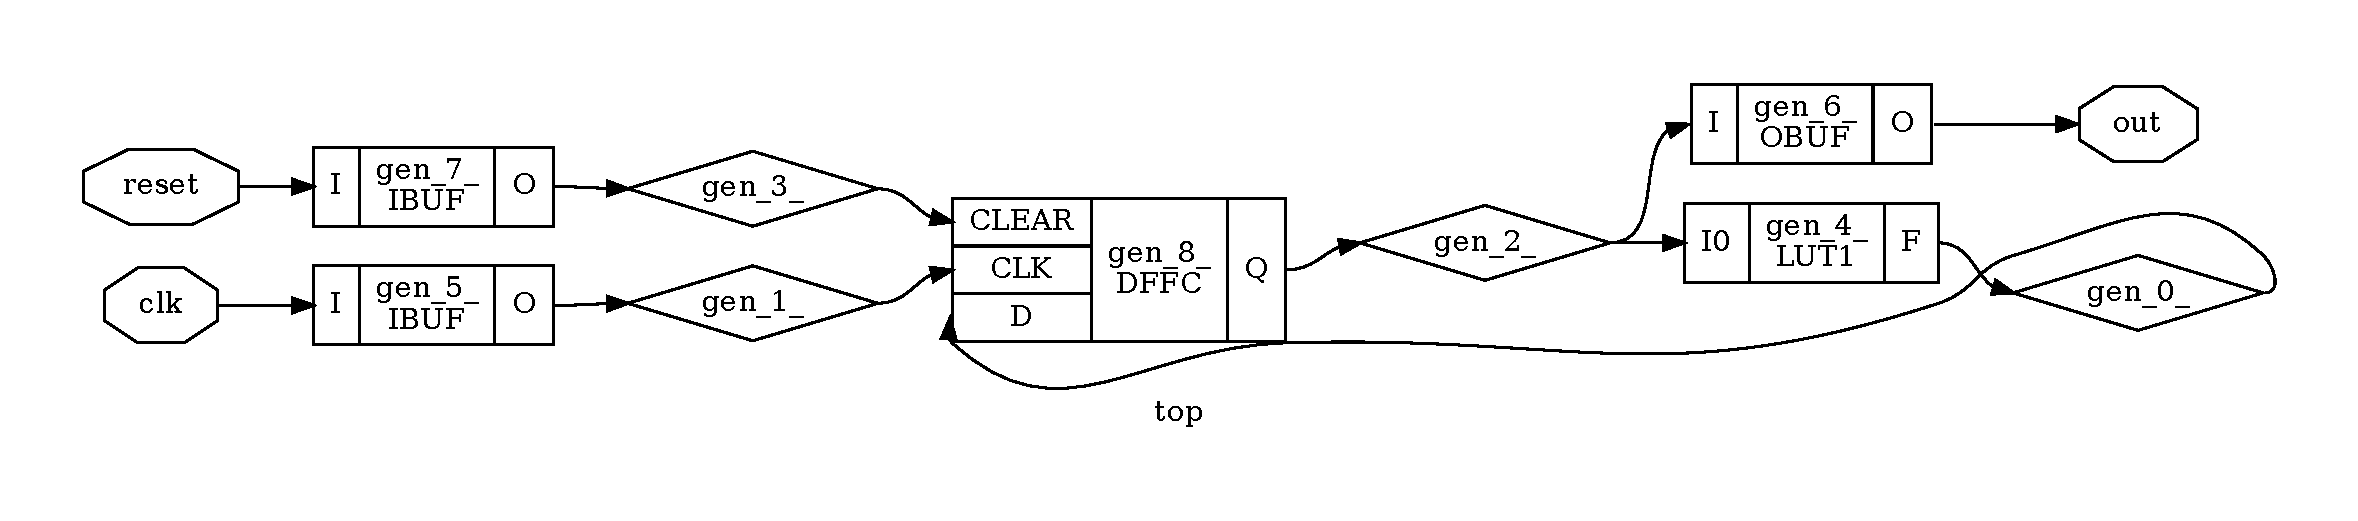
\includegraphics[width=\textwidth]{fig/post_syn.pdf}
    \caption{Post-synthesis netlist}
    \label{fig:postsynth}
\end{figure}

\begin{figure}
    \centering
    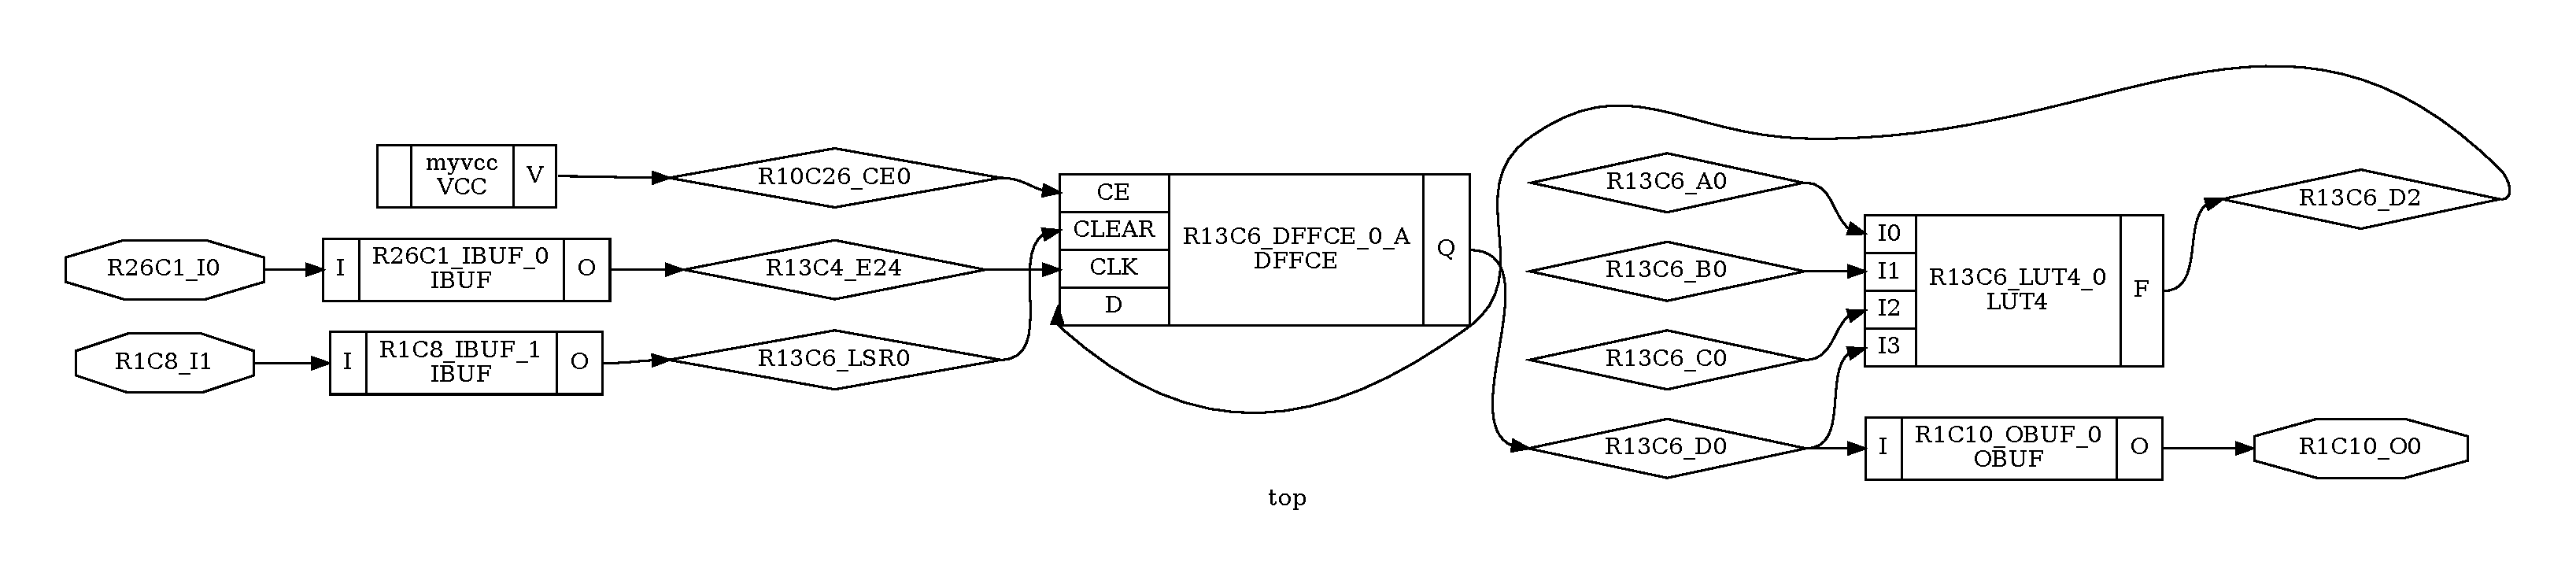
\includegraphics[width=\textwidth]{fig/post_pnr.pdf}
    \caption{Netlist unpacked from bitstream}
    \label{fig:postpnr}
\end{figure}

\subsection{Nextpnr}

Nextpnr presently has 3 targets, iCE40, ECP5, and the generic target. The final goal is to add a fourth Gowin target, implemented in C++. However, this will take thousands of lines of C++. As discussed previously, the generic target was used instead for a simple proof of concept.

The Nextpnr code includes a sample project that demonstrates how a simple imaginary FPGA could be implemented in Python. This was used as a basis for the simplified Gowin target. The major difference between the simple target and Gowin is that Gowin has much more wires and more powerful flip-flops.

This means that the reset and clock polarity features of the Gowin flip-flops are not used, and that all flip-flops within a tile share the same clock input. The generic packer packs a LUT and a DFF into a generic slice that gets mapped to the FPGA fabric, unfortunately the top two LUTs in a Gowin slice don't have a DFF, so were not used at all.

Only I/O buffer and logic tiles were used, and only in their most basic configuration. For example, buffers can also be configured for differential signaling, and logic tiles can also be configured as ALU or memory tiles. Other tile types such as BRAM, PLL, and DSP were not used at all.

The Python target is also extremely slow, taking dozens of seconds each run to load the data files. This is because in the C++ targets, these are C structures that are directly memory-mapped into RAM, whereas the Python target programmatically recreates the routing graph from the vendor data files.

To demonstrate the output of the PnR flow, a script was written that generates a netlist and post-placement file compatible with the vendor Floorplanner tool. This way the placement of tiles can be visualized. A simple blinky program reproduced in listing \ref{fig:blinky} produced the output in figure \ref{fig:floorplanner}.

\begin{figure}
    \centering
    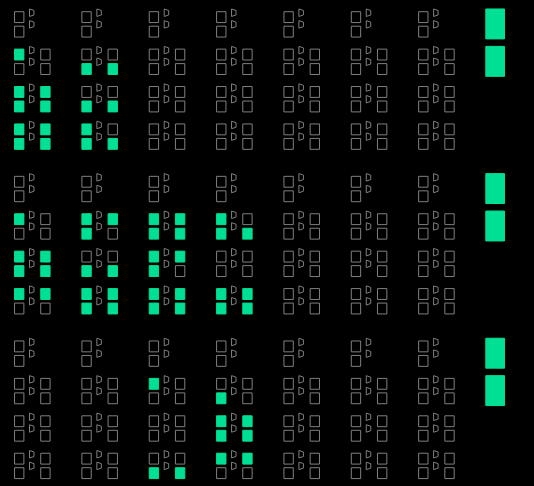
\includegraphics[width=\textwidth]{fig/floorplanner.png}
    \caption{Nextpnr results loaded in vendor Floorplanner tool}
    \label{fig:floorplanner}
\end{figure}

\begin{listing}
        \centering
\begin{minted}{verilog}
module top(input clk, output reg [7:0] leds);

reg [25:0] ctr;
always @(posedge clk)
	ctr <= ctr + 1'b1;
	
assign leds = ctr[25:18];
endmodule
\end{minted}
    \caption{Blinky code}
    \label{fig:blinky}
\end{listing}

Since the PoC Nextpnr uses the generic target rather than a custom C++ target, no major contributions to Nextpnr have been made as of yet. Instead, the Python code for the generic target is published as part of Project Apicula at \url{https://github.com/pepijndevos/apicula/tree/master/generic}.

\subsection{Bitstream packer}

The last major piece of the puzzle for an end-to-end HDL-to-bitstream flow is the bitstream packer that takes Nextpnr output and generates an FPGA bitstream. This was written in Python, reusing code from the unpacker.

Writing the packer required revisiting previously ignored details, such as the bitstream command structure and CRC verification. For the moment, an empty "donor" bitstream is used for the commands and bitstream "template", but a certain degree of understanding is required. Most importantly, each frame contains a CRC to verify the validity of the frame, but the first frame includes \textit{some} command data. There is also a file checksum, but this appears to be ignored by the FPGA.

After verifying that a vendor bitstream can be fully decoded and re-encoded with identical results and valid CRC, work began on generating the actual frame data. Despite several bugs, this was a reasonably smooth process.

\section{Demonstration of end-to-end flow}

The resulting flow was first tested by applying constant outputs on the LEDs, then by wiring the user button directly to the LEDs, then adding an inverter gate, and finally the blinky form listing \ref{fig:blinky}. The first ever end-to-end open source blinky program running on a Gowin FPGA is shown in figure \ref{fig:trenzblinky}.

It was theorized that because global clock routing was not yet implemented, nontrivial designs would face severe clock skew leading to timing violations. On the other hand it was argued that these smaller, more low-power devices are a lot more forgiving than larger high-performance parts.

To put this hypothesis to the test, a RISV-V CPU was synthesized. For this task the PicoRV32 was chosen in the AttoSoC configuration. This configuration is very minimal and does not have any memory besides the registers, making it suitable for the current flow that does not yet have block RAM.

For the software, a simple program was chosen that calculates all primes under 256 and displays them in binary on the LEDs of the FPGA. The code can be found in listing \ref{fig:prime}. The whole AttoSoC design was synthesized with Yosys, using 5099 out of  6480 FPGA slices, 78\% of the available resources, taking into account only 3/4 of the slices can be used in the current flow due to limitations in the \texttt{nextpnr-generic} packer.

The design was then placed and routed in Nextpnr, taking 234 placer iterations and 408985 routing interactions, taking several minutes to complete. The generated \texttt{.posp} file was then loaded in the Gowin floorplanner, shown in figure \ref{fig:picorv}. As can be seen, almost the full FPGA is utilized by this design, but all of the DSP and BRAM blocks are left untouched.

The resulting JSON file was then packed into a bitstream, and programmed using the Gowin JTAG programmer. The design ran correctly at \SI{12}{\mega\hertz} on the first try, showing that complex designs can be used with the current flow. In figure \ref{fig:riscprime}, the Gowin FPGA is seen displaying the numbers 37, 47, 61 and 73 in decimal, which are indeed prime.

\begin{figure}
    \centering
    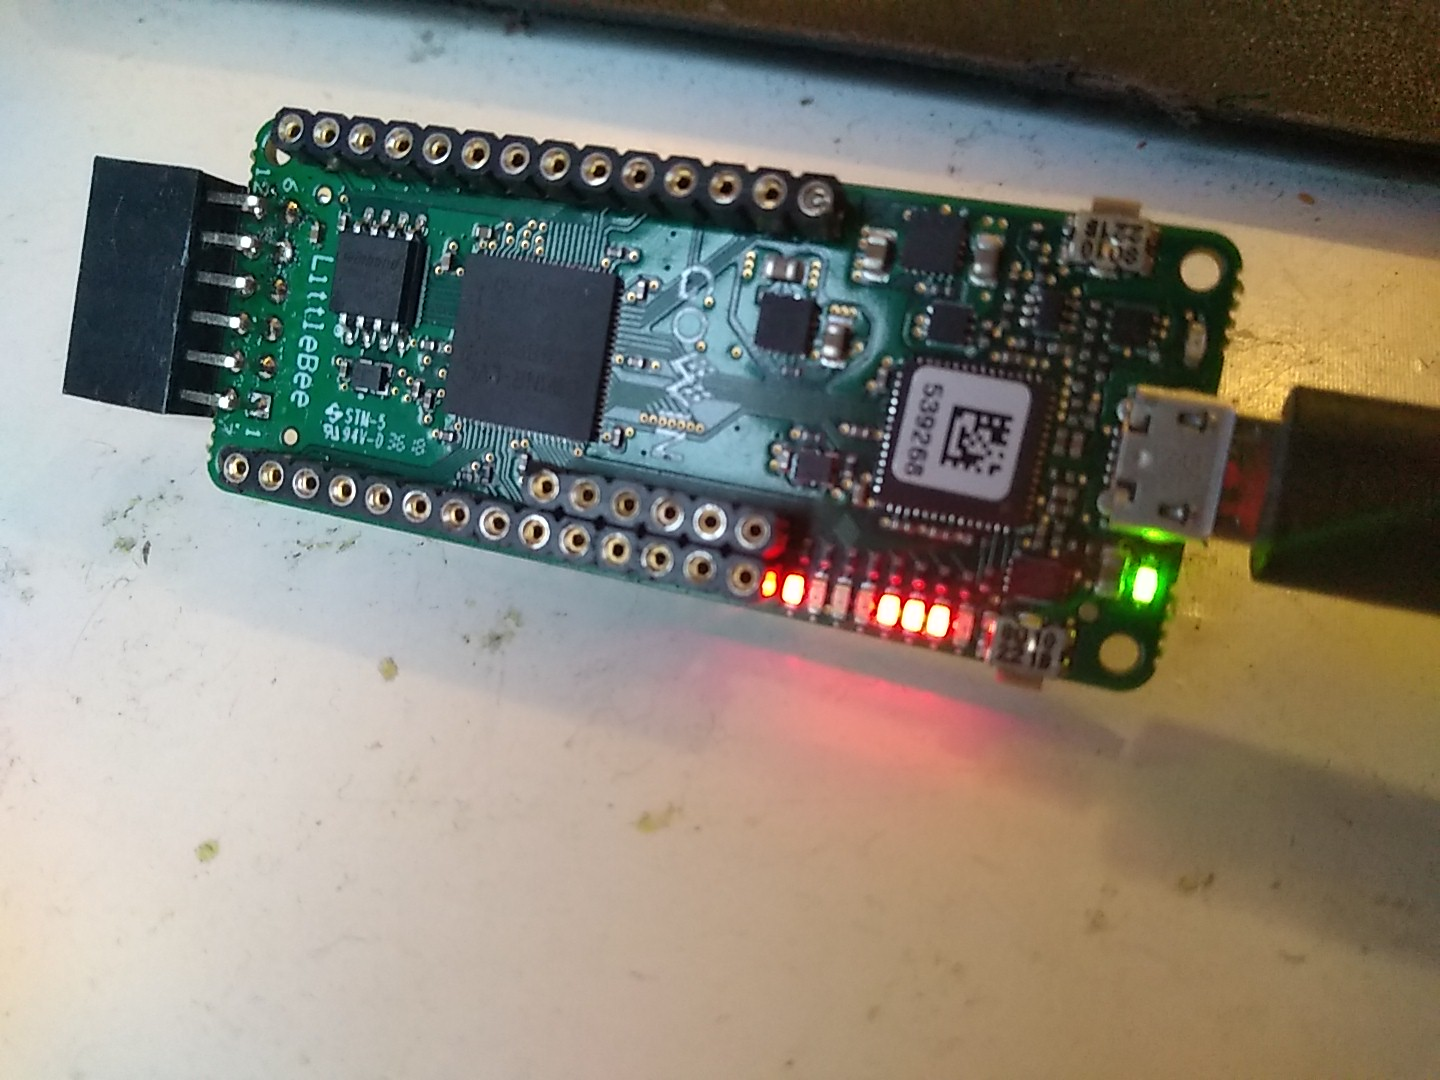
\includegraphics[width=0.8\textwidth]{fig/blinky.jpg}
    \caption{First end-to-end open source blinky running on a Gowin FPGA}
    \label{fig:trenzblinky}
\end{figure}

\begin{figure}
    \centering
    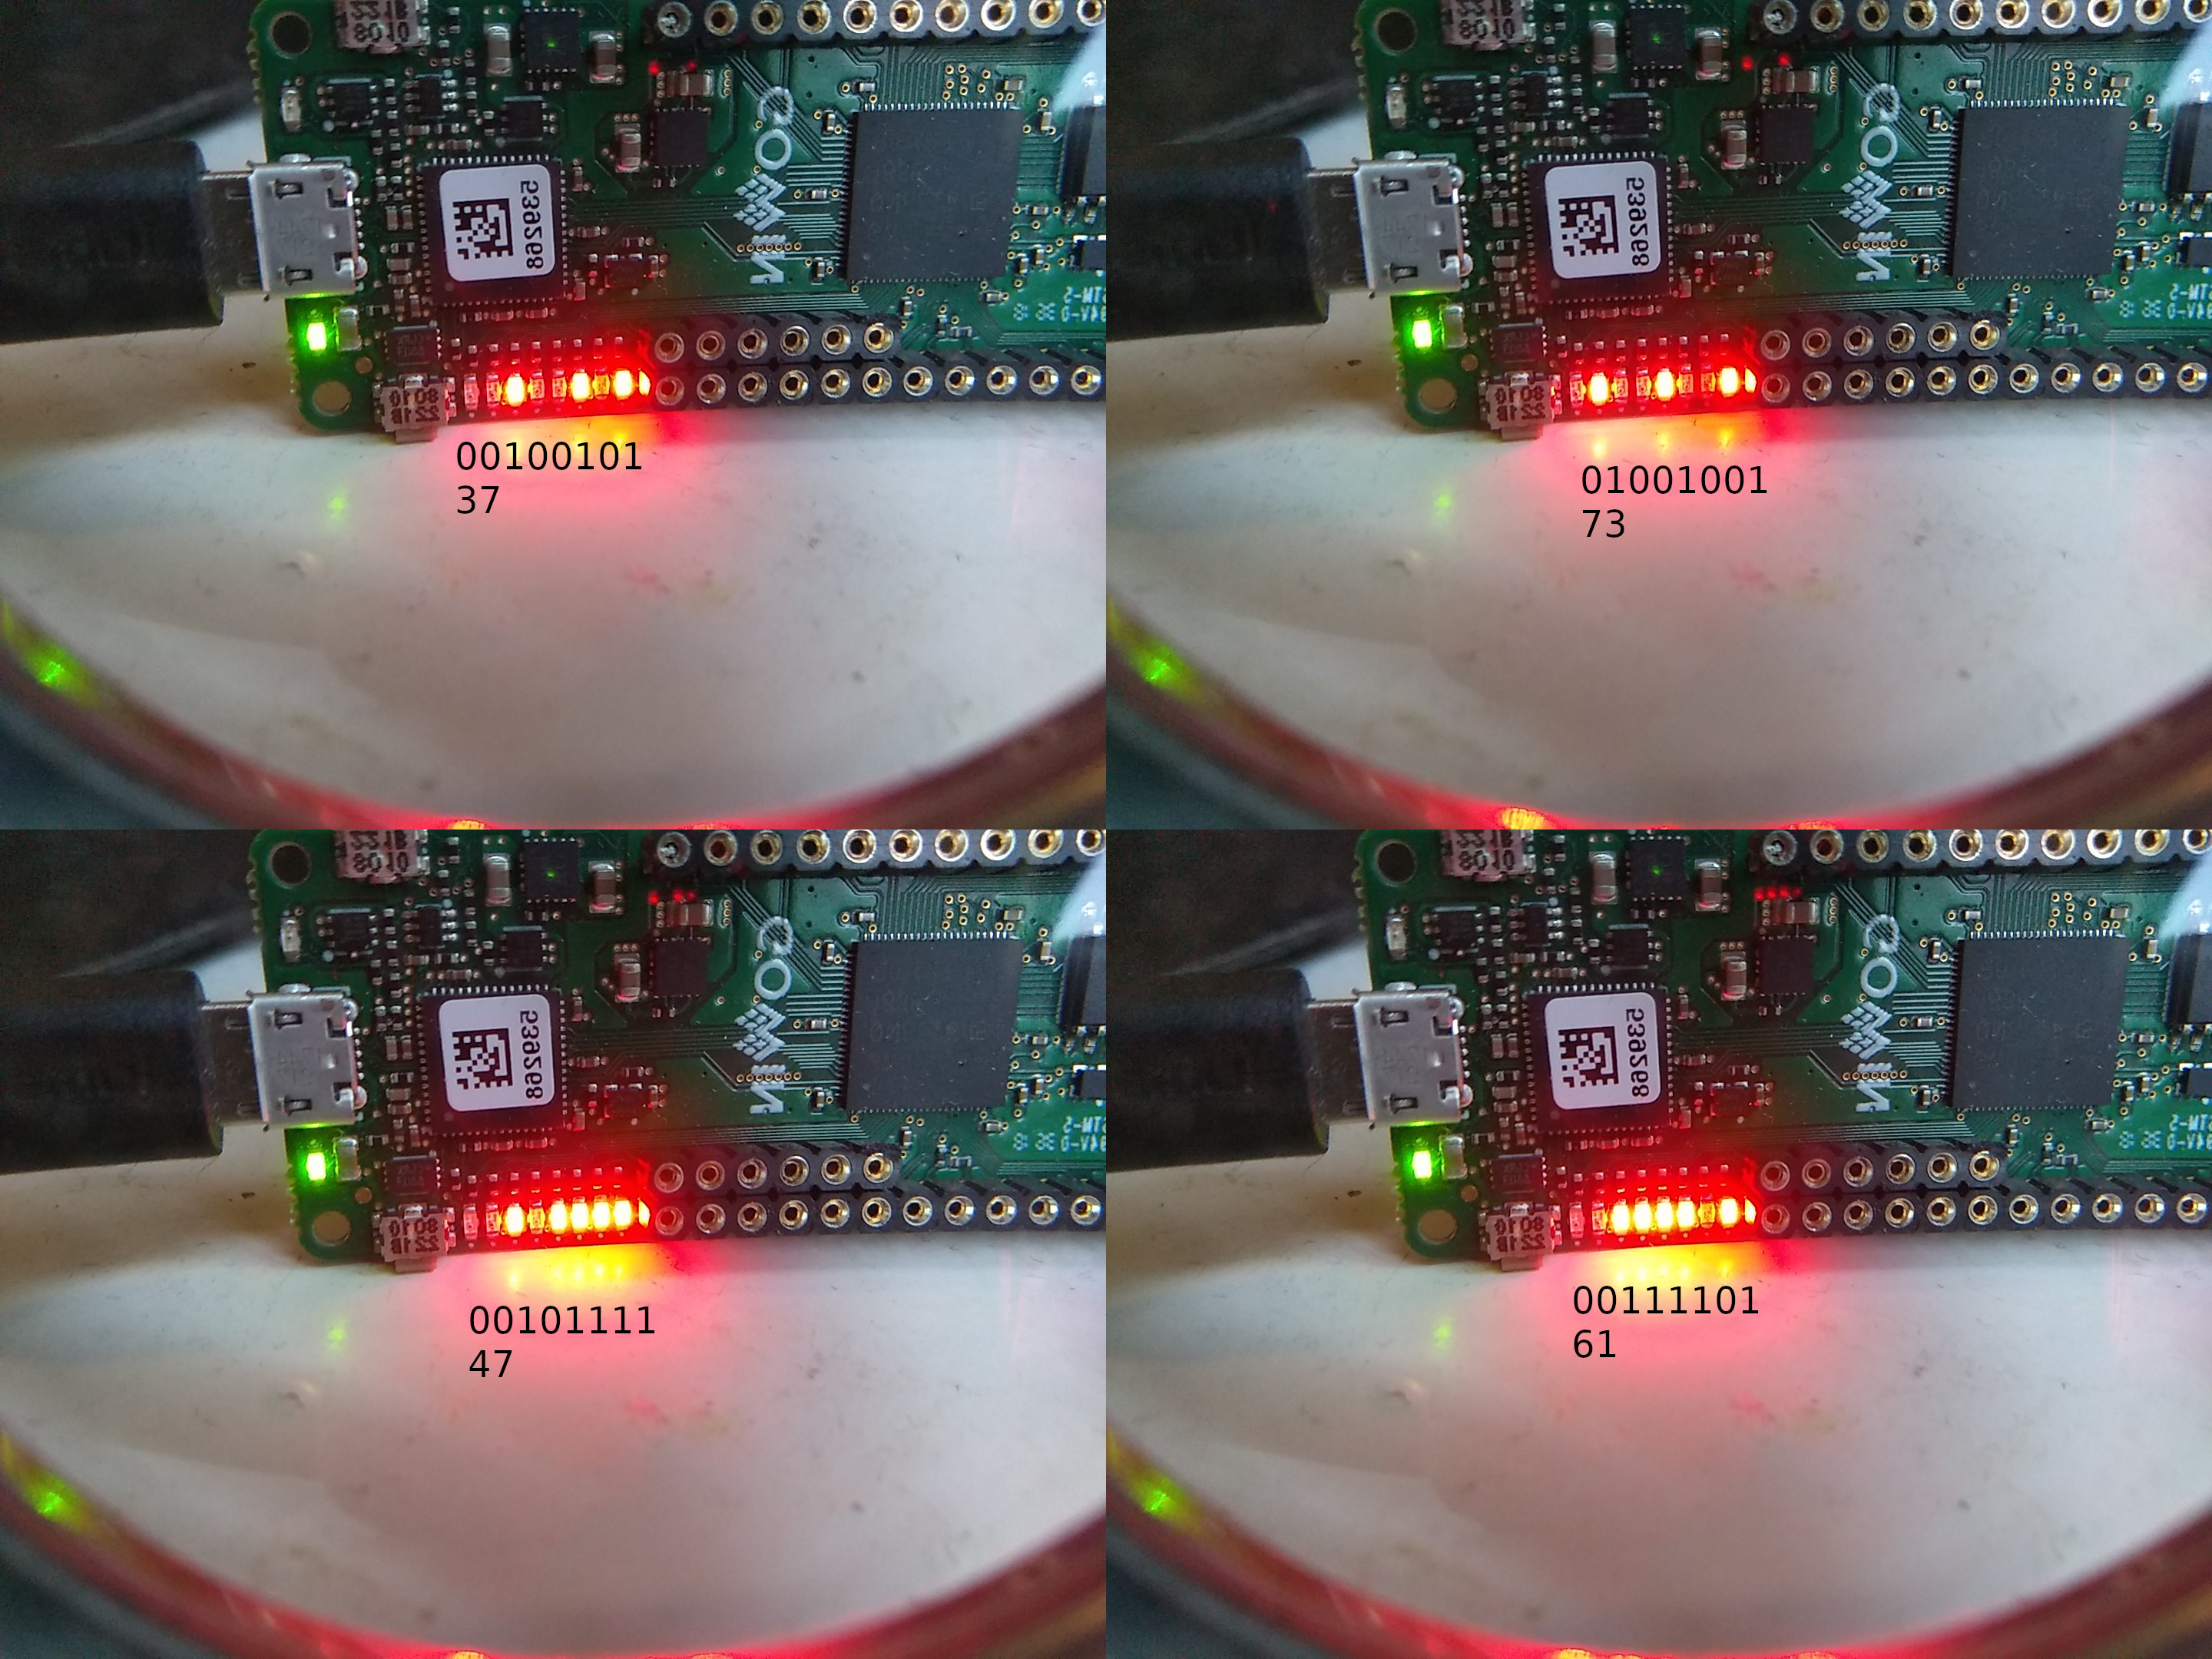
\includegraphics[width=0.8\textwidth]{fig/primes.jpg}
    \caption{End-to-end open source RISC-V prime calculation running on a Gowin FPGA}
    \label{fig:riscprime}
\end{figure}

\begin{figure}
    \centering
    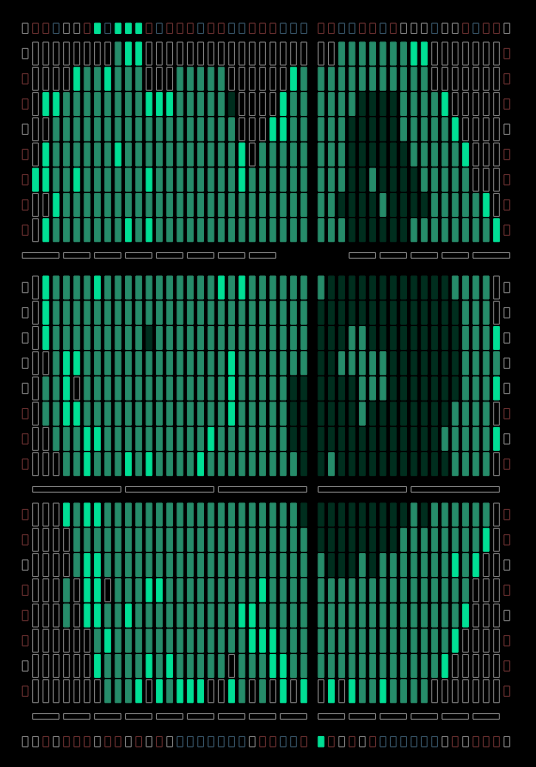
\includegraphics[width=\textwidth]{fig/picorv.png}
    \caption{PicoRV32 routed with Nextpnr shown in Gowin Floorplanner}
    \label{fig:picorv}
\end{figure}

\begin{listing}
        \centering
\begin{minted}{gas}
start:
    li s0, 2
    li s1, 0x02000000
    li s3, 256
outerloop:
    addi s0, s0, 1
    blt s0, s3, inrange
    li s0, 2
inrange:
    li s2, 2
innerloop:
    bge s2, s0, prime
    add a0, s0, 0
    add a1, s2, 0
    jal ra, divtest
    beq a0, x0, notprime
    addi s2, s2, 1
    j innerloop
prime:
    sw s0, 0(s1)
    jal ra, delay
notprime:
    j outerloop

divtest: 
    li t0, 1
divloop:
    sub a0, a0, a1
    bge a0, t0, divloop
    jr ra
    
delay:
    li t0, 360000
delayloop:
    addi t0, t0, -1
    bnez t0, delayloop
    jr ra
\end{minted}
    \caption{Prime code \cite{prime}}
    \label{fig:prime}
\end{listing}

\section{Conclusion and future work}

With the goal of adding support for Gowin FPGAs to Yosys and Nextpnr in mind, this report demonstrates the progress that has been made documenting the Gowin FPGA architecture and bitstream format and writing open source tools for these FPGAs.

Yosys support for Gowin FPGAs was extended to the point where it almost covers all primitives that the vendor supports, with the exception of latches, DSP, and some primitives that cannot be automatically inferred by Yosys. This support has been merged upstream in \url{https://github.com/YosysHQ/yosys/pull/1449}, and can be used already with the vendor tools for PnR.

The basic architecture of the FPGA and the structure of the bitstream were described, including the topology of inter-tile wires, the layout of the tiles, and bit locations controlling basic primitives. An unpacker was written to decode simple designs from a bitstream file to show that the basic logic and routing are correctly understood.

A proof of concept Nextpnr target and bitstream packer were written to demonstrate a fully open source flow capable of synthesizing and running various programs. It was shown that the open source flow is capable of synthesizing a full RISC-V CPU that works correctly on a GW1NR-9 FPGA. This demonstrates that even at this early stage, the open source flow can be used for relatively complex software, as long as it does not place high requirements on memory and DSP.

However, at this moment, many features of the FPGA remain unexplored. Up to this point, the main focus has been on understanding the configurable logic tiles and routing fabric. In this area, global clock nets, long wires, ALU modes, and DRAM memory modes remain unexplored.

Other tile types have received a lot less focus. For IOB tiles, only a bare minimum is supported. Much work remains to be done for more complicated usage such as tri-state outputs, differential pairs, and different drive strengths and levels. Other tiles such as DSP, BRAM and PLL, are completely unexplored.

So far, a lot has been achieved, but a long road lays ahead before mature Gowin support is implemented in Yosys and Nextpnr.

\printbibliography


\end{document}
